\documentclass[11pt,a4paper]{report}

\usepackage[T1]{fontenc}
\usepackage{lmodern}
\usepackage{amsmath}
\usepackage{amssymb}
\usepackage{amsthm}
\usepackage{graphicx}
\usepackage{booktabs}
\usepackage{caption}
\usepackage{geometry}
\usepackage{enumitem}
\usepackage{xcolor}
\usepackage{microtype}
\usepackage{textcomp}
\providecommand{\arcsec}{\ensuremath{^{\prime\prime}}}
\usepackage[hidelinks]{hyperref}

\geometry{a4paper, margin=2.5cm}

\hypersetup{
  colorlinks=true,
  linkcolor={black!75!blue},
  citecolor={black!70!green},
  urlcolor={black!55!blue},
  pdftitle={structure-first-ml -- Collected Technical Reports},
  pdfauthor={Enes Oz}
}

\graphicspath{{figs/}}
\captionsetup{font=small, labelfont=bf, width=0.9\textwidth}

\newcommand{\sig}{\mathbf{S}}
\newcommand{\R}{\mathbb{R}}
\newtheorem{theorem}{Theorem}
\newtheorem{definition}{Definition}

\linespread{1.05}
\setlength{\parskip}{0.4em}
\emergencystretch=3em
\hbadness=10000

\begin{document}

\begin{titlepage}
\centering
\vspace*{2.2cm}
{\Large\scshape structure-first-ml}\\[0.6cm]
\rule{0.72\textwidth}{0.4pt}\\[0.8cm]
{\huge\bfseries Collected Technical Reports\par}
\vspace{0.9cm}
{\large Structure-first machine learning for physical data\par}
\vspace{1.6cm}
{\large\bfseries Enes \"Oz\par}
\vspace{0.4cm}
{\normalsize Independent research project\par}
\vspace{0.3cm}
{\normalsize Draft --- July 2026\par}
\vspace{2.0cm}
\begin{minipage}{0.82\textwidth}
\small
\noindent\textbf{Preface.} Most machine-learning pipelines coerce data into the shape the
model expects: irregular observations are interpolated onto a regular grid, point clouds are
voxelised, curved domains are flattened, and conserved quantities are left to be learned by
accident. Each step discards structure that was present in the measurement and introduces
artefacts that were not. The work collected here reverses that order of reasoning ---
identify the mathematical object the data belongs to, choose a representation with the
invariances that object actually has, and only then attach a learning algorithm. Where the
representation carries a theorem, the theorem is stated and its hypotheses are tested against
real data rather than assumed. Results are reported in both directions: the cases where the
approach wins and the cases where it loses are given equal space, because a representation
that is claimed to help everywhere has not been understood anywhere.
\end{minipage}
\vfill
{\small Data courtesy of the Zwicky Transient Facility, the ZTF Bright Transient Survey, the
ALeRCE broker, the Global Meteor Network (CC~BY~4.0) and the IAU Meteor Data Center.\par}
\end{titlepage}

\tableofcontents
\clearpage

\chapter{Path signatures for irregularly sampled light curves}
\label{ch:t1}
\noindent\textit{projects/t1-signature-lightcurves}

\section*{Abstract}
\addcontentsline{toc}{section}{Abstract}

A photometric light curve is a finite sample of a path, not a vector: observations arrive at
times set by weather and scheduling, in whichever filter was in use, with per-point
uncertainties varying by an order of magnitude. Standard pipelines destroy that structure at
the first step by interpolating onto a regular grid. The signature transform of rough path
theory consumes the raw stream directly and is invariant under reparameterisation of time.
This chapter tests whether that theoretical advantage survives contact with real survey
photometry, on 2{,}375 spectroscopically classified ZTF transients in eight classes. The
answer is qualified, and the qualifications are the substance of the chapter.

\section{Introduction}

The signature of a path has been applied once in astronomy, to radio-frequency interference
detection in interferometric visibility streams \cite{signova}. Time-domain photometric
classification is untouched. That gap is narrow enough to be worth attempting and broad
enough to be worth reporting either way.

The incumbent methods are not weak. Hand-crafted variability features in the lineage of FATS
and \texttt{feets} have absorbed two decades of domain knowledge; Gaussian-process
interpolation is the principled treatment of irregular sampling; random convolutional kernel
methods such as MiniRocket \cite{minirocket} are cheap, deterministic and strong. A new
representation earns its place only by beating these or by adding something they lack.

\section{Mathematical background}

\begin{definition}[Signature]
For a continuous path $X : [0,T] \to \R^d$ of bounded variation, the signature is the
sequence of iterated integrals
\[
\sig(X) \;=\; \left(1,\; \int_{0<t<T}\!\mathrm{d}X_t,\;
\iint_{0<s<t<T}\!\mathrm{d}X_s \otimes \mathrm{d}X_t,\; \dots \right),
\]
whose $k$-th term is an element of $(\R^d)^{\otimes k}$.
\end{definition}

Three properties motivate its use here.

\paragraph{Reparameterisation invariance.} For any increasing reparameterisation
$\varphi$, $\sig(X \circ \varphi) = \sig(X)$. The signature encodes the order and shape of
what happened, not the clock on which it happened. When observation times are set by the
weather rather than by the source, this is the correct invariance to have; interpolation-based
pipelines must learn it from data instead.

\paragraph{Faithfulness.} The signature determines the path up to tree-like equivalence,
informally up to retracing \cite{hambly}. Nothing is discarded but the parameterisation.

\paragraph{Universality.} Linear functionals of the signature approximate continuous functions
on path space uniformly on compact sets. A linear model on signature features is therefore a
universal approximator on paths, which converts architecture design into a question of
truncation depth.

For a piecewise-linear path the signature has a closed form. Each straight segment with
increment $\delta$ contributes the tensor exponential $\delta^{\otimes k} / k!$ at level $k$,
and segments concatenate by Chen's identity
\[
\sig(X * Y)_k \;=\; \sum_{i=0}^{k} \sig(X)_i \otimes \sig(Y)_{k-i}.
\]
Truncating at depth $m$ retains $\sum_{k=1}^{m} d^k$ coefficients.

\subsection{Implementation and verification}

The transform is implemented from scratch rather than imported, because the theory track
requires access to individual tensor levels and because the standard C\texttt{++} backends do
not build reliably on current Python versions. Correctness is established two ways: agreement
with \texttt{esig}, \texttt{signax} and \texttt{roughpy} to $\sim10^{-13}$ across four path
configurations, and four structural identities checked directly --- reparameterisation
invariance, level one equalling the total increment, the shuffle identity
$S_1 S_2 = S_{12} + S_{21}$, and the vanishing of the signature of a path concatenated with
its own reversal. All sixteen checks pass.

\section{Where the ordering information lives}
\label{sec:order}

Before applying the transform to real data it is worth confirming that the claimed mechanism
exists, in a setting where the answer follows from the construction. Two classes of synthetic
double-peaked light curve are built to differ only in which peak comes first: the peaks sit
symmetrically about the midpoint of the window and the curve starts and ends at the same
baseline, so one class is the exact time reverse of the other. The marginal distribution of
magnitudes is therefore identical between classes, and so is the net change from first to last
observation.

The prediction recorded in advance was that separation would appear at depth 2, the Lévy area
being the classical order-sensitive term. It does not.

\begin{table}[h]
\centering
\small
\begin{tabular}{lr}
\toprule
Representation & Balanced accuracy \\
\midrule
Order-blind summary features & 0.512 \\
Signature depth 1 & 0.524 \\
Signature depth 2 & 0.489 \\
Signature depth 3 & \textbf{0.978} \\
Signature depth 4 & 0.990 \\
\bottomrule
\end{tabular}
\caption{Separation of two synthetic classes differing only in the order of two peaks.
Chance is 0.5. Ordering becomes visible at level 3, not level 2.}
\end{table}

The reason is geometric and specific to this path construction. With channels
$(t, m)$ the time coordinate is strictly increasing, so the antisymmetric part of level 2 ---
the Lévy area --- reduces to $\int m \,\mathrm{d}t$ once the boundary terms vanish. That is the
area under the light curve, which is the same whichever peak came first. A path monotone in one
coordinate encloses no signed area that ordering can change. Ordering first becomes visible at
level 3, in terms of the form $\iiint \mathrm{d}t\,\mathrm{d}m\,\mathrm{d}t$, which weight
magnitude excursions by when they occurred.

The practical consequence is direct: truncating at depth 2 to economise on features would
discard precisely the information the method exists to supply, and the resulting null result
would have been attributed to the astrophysics.

\section{Data}

Labels are the spectroscopic classifications of the ZTF Bright Transient Survey; per-epoch
photometry in $g$ and $r$ is served by the ALeRCE broker. ALeRCE's own machine
classifications are never used, since training on one classifier's output and reporting
agreement with it measures nothing.

After quality cuts requiring at least ten detections and at least three in each band, the
sample is 2{,}375 objects with a median of 42 detections spanning a median of 122 days, in
eight classes: CV (456), SN~II (426), SN~Ia (406), AGN (376), SN~IIn (273), SN~Ic (185),
SN~Ib (148) and SLSN-I (105).

A first version of the fetch submitted objects grouped by class while the broker's failure
rate rose during the run, so classes submitted last lost far more objects than those submitted
first and SN~Ib was eliminated entirely. That is a selection effect on the label rather than
random attrition, and it would have corrupted every downstream number. After shuffling before
any network call, lowering concurrency and adding exponential backoff, the per-class retrieval
rate is 1.0 across all eight classes.

\begin{figure}[h]
\centering
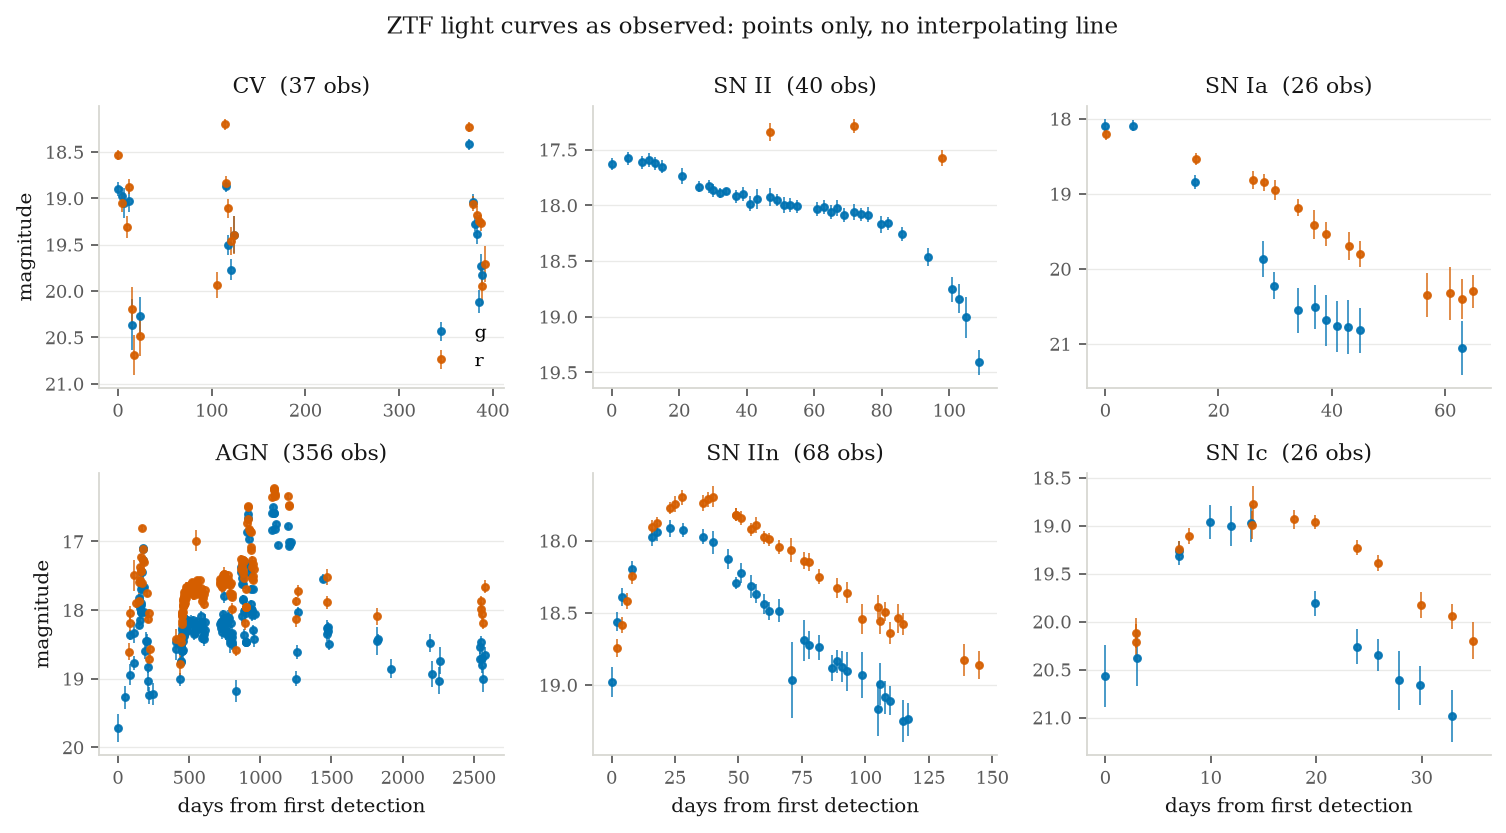
\includegraphics[width=\textwidth]{fig1_lightcurves.png}
\caption{Example light curves, one per class, drawn as points with error bars and no
connecting line: a line between observations would assert a continuity the data does not
contain. Note the range of durations, from 26 detections over 65 days to 356 over 2{,}500.}
\end{figure}

\begin{figure}[h]
\centering
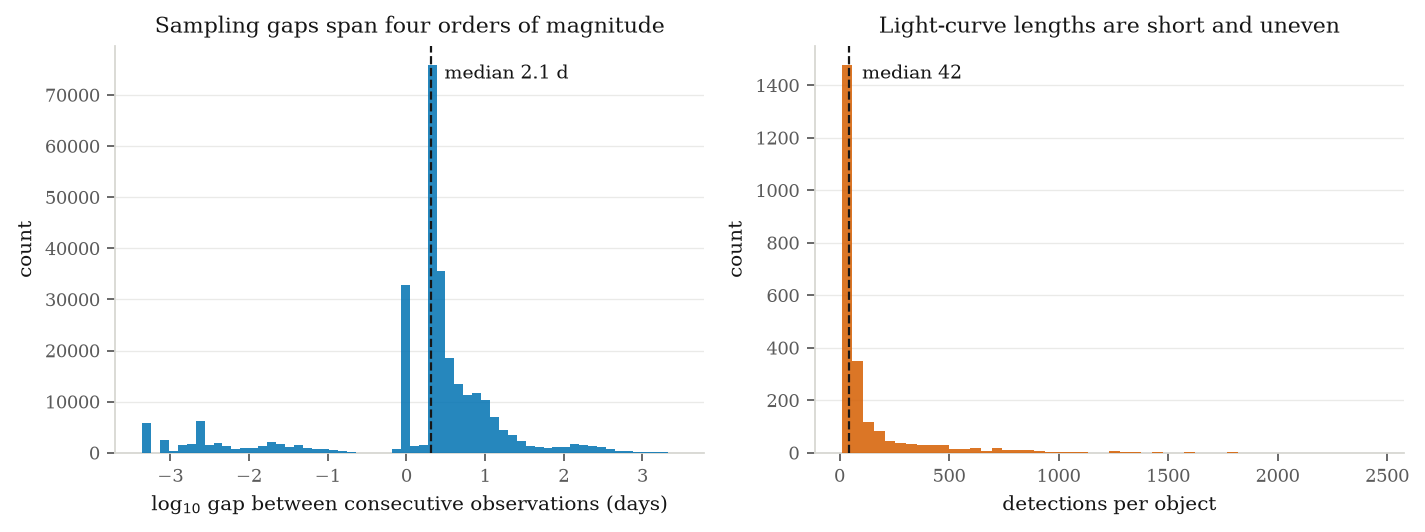
\includegraphics[width=\textwidth]{fig2_sampling.png}
\caption{The sampling gap distribution is bimodal and spans four orders of magnitude:
repeated exposures within a single night near $10^{-3}$ days, the main survey cadence at 1 to
10 days, and seasonal visibility windows at 100 to 1{,}000 days. Same-night exposures occupy
almost no arc length and so barely move the signature, whereas a fixed-grid method weights
them like any other sample.}
\end{figure}

\section{Method}

\subsection{Constructing the path}

The difficult part is not the signature but deciding what the path is. Observations in
different filters are not simultaneous, so no instant exists at which a two-band vector is
defined, and any joint multi-channel construction embeds a choice. Three are implemented and
compared rather than assumed: \emph{per-band}, in which each filter is its own
two-dimensional path and the signatures are concatenated, with no cross-band information and
no interpolation; \emph{interleaved}, in which all observations in time order form one path
with a band indicator channel; and \emph{joint forward-fill}, a common time axis with the last
observed magnitude carried forward, which is piecewise-constant interpolation and is labelled
as such.

\subsection{Channel preparation}

How the channels are prepared turned out to matter more than which path construction was
used. Scaling time to $[0,1]$ discards the duration of the event; centring magnitudes discards
absolute brightness. Both are strong physical discriminants for transients, and the
hand-crafted baseline retains them as \texttt{t\_span} and \texttt{peak\_mag}. Discarding them
and then reporting that signatures lose would measure the preprocessing rather than the
representation.

A related fact is worth stating because it is a check on the implementation rather than a
result: the \emph{raw} and \emph{raw time} preparations score identically to four decimal
places. The signature depends only on increments, so a constant magnitude offset cannot change
it. Absolute brightness can enter only through a basepoint, and when introduced that way it
degrades performance rather than improving it.

\subsection{Baselines}

Every representation is evaluated on identical cross-validation folds with identical
classifiers. The hand-crafted baseline implements the FATS and \texttt{feets} lineage from
scratch; almost all of its features are functions of the marginal magnitude distribution and
are therefore invariant to permuting observations in time, which is exactly the information
signatures retain. The three ordering-sensitive features it does contain --- linear trend, rise
and fade fractions, maximum slope --- are included deliberately, since omitting them would make
the comparison dishonest. MiniRocket is given linearly interpolated fixed-length input, which
is its best case; that interpolation is precisely the cost the signature approach claims to
avoid, and granting the baseline its best case is the only way to measure that cost.

\section{Results}

All figures are balanced accuracy under stratified cross-validation with gradient-boosted
trees, on 2{,}375 objects in eight classes. Chance is 0.125.

\subsection{Preprocessing dominated the representation}

\begin{table}[h]
\centering
\small
\begin{tabular}{lrr}
\toprule
Representation & Features & Balanced accuracy \\
\midrule
summary $+$ signature (lead-lag, depth 4) & 729 & \textbf{0.578} \\
summary (hand-crafted) & 49 & 0.560 \\
signature, per-band, raw time, lead-lag, depth 4 & 680 & 0.548 \\
MiniRocket (interpolated grid) & 9{,}996 & 0.538 \\
signature, per-band, raw time, depth 4 & 60 & 0.524 \\
signature, per-band, unit time, depth 4 & 60 & 0.455 \\
\bottomrule
\end{tabular}
\caption{Head-to-head comparison. The gap between the last two rows is the cost of
discarding event duration by scaling time to $[0,1]$; the gap between rows three and five
is the gain from the lead-lag transform.}
\end{table}

Scaling time to $[0,1]$ costs 0.069, because it discards the duration of the event, which
the hand-crafted baseline retains as \texttt{t\_span}. The first version of this pipeline
did exactly that, and would have reported a far worse number as a property of signatures
rather than of the preprocessing. The lead-lag transform is worth a further 0.025, taking
signatures past MiniRocket but not past the incumbent; it exposes quadratic variation, and
roughly a third of the sample (AGN and CV) is stochastically variable rather than transient.

A third observation is a check on the implementation rather than a result: the \emph{raw}
and \emph{raw time} preparations score identically to four decimal places. The signature
depends only on increments, so a constant magnitude offset cannot change it. Absolute
brightness can enter only through a basepoint, and introduced that way it degrades
performance rather than improving it.

\subsection{Complementarity, with a matched-noise control}

Signatures alone lose to a 49-feature baseline while using fourteen times as many features.
The concatenation scores above the baseline, but by 0.015 against a fold spread of 0.020,
which on its own establishes nothing. The question was therefore given a dedicated test:
fifty paired folds on identical splits, a Wilcoxon signed-rank test, a bootstrap interval,
and a control in which the signature block is replaced by Gaussian noise of identical shape
and column variance.

\begin{table}[h]
\centering
\small
\begin{tabular}{lr}
\toprule
Feature block & Balanced accuracy \\
\midrule
summary $+$ signature & $\mathbf{0.5769 \pm 0.0200}$ \\
summary & $0.5623 \pm 0.0167$ \\
signature alone & $0.5473 \pm 0.0218$ \\
summary $+$ matched noise & $0.5278 \pm 0.0146$ \\
\bottomrule
\end{tabular}
\hspace{1em}
\begin{tabular}{lrr}
\toprule
vs.\ summary & Difference & Folds improved \\
\midrule
$+$ signature & $+0.0147$ & 38 / 50 \\
$+$ matched noise & $-0.0345$ & 1 / 50 \\
\bottomrule
\end{tabular}
\caption{Left: mean and standard deviation across fifty paired folds. Right: paired
differences against the baseline, with 95\% bootstrap intervals $[+0.0078, +0.0212]$ and
$[-0.0396, -0.0297]$ respectively.}
\end{table}

The control is what makes the result readable. A gradient-boosted ensemble handed 680 extra
candidate splits might improve for reasons unrelated to their contents; it does not. Six
hundred and eighty columns of noise \emph{cost} 0.0345, while the same number of signature
columns \emph{gain} 0.0147, under identical folds and identical dependence structure.

One caveat belongs beside the $p$-value ($9.5 \times 10^{-5}$): repeated cross-validation
folds reuse the same 2{,}375 objects and are not independent, so both it and the bootstrap
interval are optimistic as formal inference. The comparison that does not rest on that
assumption is the one against the noise control, and it is the one the conclusion leans on.

\subsection{The sampling ablation}

The headline accuracy on full light curves says little, because every representation does
reasonably well when the data are dense. The claim under test concerns \emph{where}
signatures should help, so the light curves were thinned to fixed retained fractions under
two regimes removing the same number of observations while destroying different structure:
\emph{random} thinning, with each observation dropped independently, and \emph{blocked}
thinning, with contiguous runs removed to imitate weather outages and seasonal windows.

\begin{table}[h]
\centering
\small
\begin{tabular}{lrrrrrrr}
\toprule
& \multicolumn{4}{c}{random} & \multicolumn{3}{c}{blocked} \\
\cmidrule(lr){2-5}\cmidrule(lr){6-8}
Representation & 1.00 & 0.60 & 0.35 & 0.20 & 0.60 & 0.35 & 0.20 \\
\midrule
summary & 0.560 & 0.549 & 0.532 & 0.513 & 0.536 & 0.520 & 0.498 \\
signature & 0.538 & 0.519 & 0.497 & 0.503 & 0.508 & 0.487 & 0.462 \\
MiniRocket & 0.538 & 0.504 & 0.478 & 0.467 & 0.481 & 0.431 & \textbf{0.398} \\
\bottomrule
\end{tabular}
\caption{Balanced accuracy against retained fraction under both thinning regimes.}
\end{table}

\begin{figure}[h]
\centering
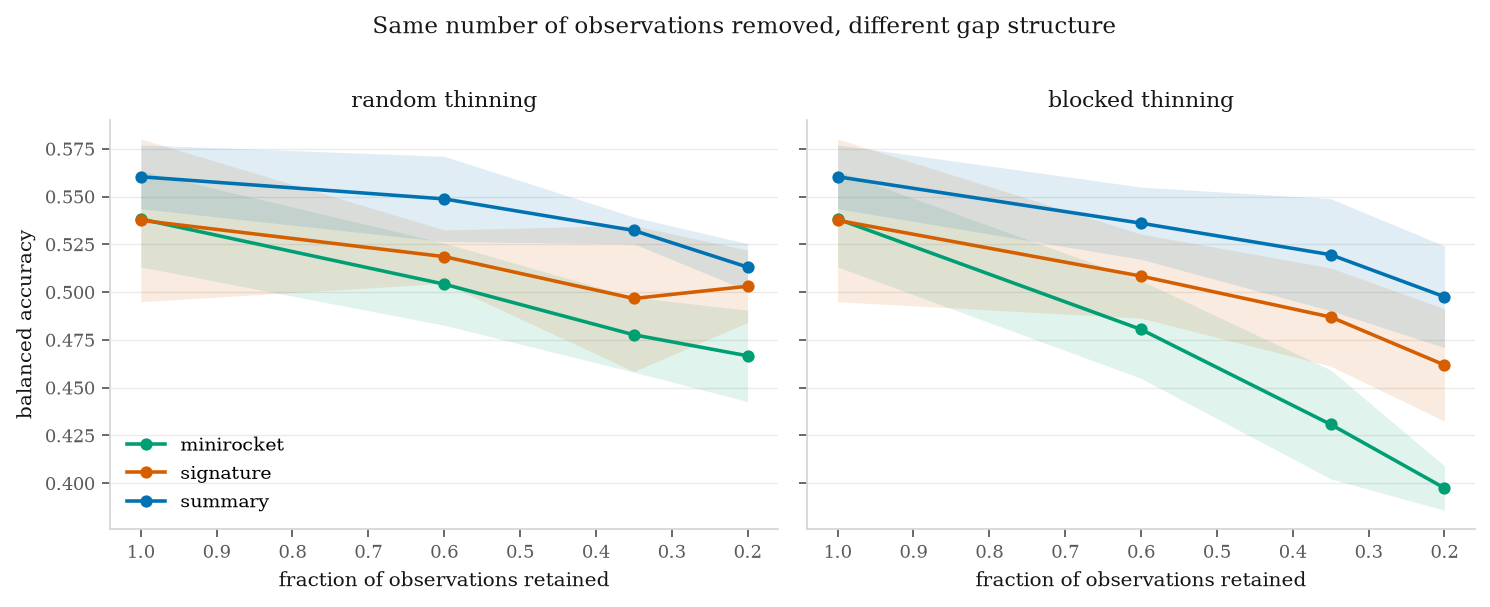
\includegraphics[width=\textwidth]{fig4_ablation.png}
\caption{The same number of observations removed under two gap structures. MiniRocket,
which requires a regular grid and is given one, collapses under blocked thinning while the
other two degrade gently.}
\end{figure}

The informative quantity is the difference between regimes at matched density --- the cost
of gap \emph{structure} with gap \emph{count} held fixed:

\begin{table}[h]
\centering
\small
\begin{tabular}{lrrr}
\toprule
Retained fraction & summary & signature & MiniRocket \\
\midrule
0.60 & $-0.013$ & $\mathbf{-0.010}$ & $-0.024$ \\
0.35 & $-0.013$ & $\mathbf{-0.010}$ & $-0.047$ \\
0.20 & $\mathbf{-0.016}$ & $-0.041$ & $-0.069$ \\
\bottomrule
\end{tabular}
\caption{Structured-gap penalty: blocked minus random at equal retained fraction.}
\end{table}

Gap structure matters, not merely gap count, and it costs the interpolation-dependent
method the most. MiniRocket pays two to four times the penalty of the other two at every
density, losing 0.069 to structured gaps alone at 20\% retention. This is the strongest
evidence in the chapter for the premise that resampling irregular data onto a grid discards
information, and it is a prediction that could have failed: identical curves under the two
regimes would have collapsed the motivation entirely.

At moderate thinning the signature is the least damaged by gap structure, which is the
direction the reparameterisation argument predicts. At the sparsest setting it is not: its
own structured-gap penalty jumps to $-0.041$, worse than the baseline's $-0.016$. Below
roughly a dozen observations per object the path is too coarsely sampled for the iterated
integrals to be estimated stably, and the invariance argument stops paying.

\subsection{The Gaia counter-test}

The counter-test was registered with the main experiment and run afterwards on 2{,}999 Gaia
DR3 periodic variables in six classes. Its logic is that ZTF transients are separated by the
shape and ordering of the light curve, which signatures encode, whereas Gaia periodic
variables are separated by \emph{period}, which is a statement about the clock --- and the
signature is invariant to reparameterisation of the clock.

\begin{table}[h]
\centering
\small
\begin{tabular}{lrr}
\toprule
Measurement & Gaia (2{,}999) & ZTF (2{,}375) \\
\midrule
Baseline minus best signature & $\mathbf{+0.0743}$ & $+0.0123$ \\
Value of keeping duration & $+0.0387$ & $\mathbf{+0.0688}$ \\
Value of the lead-lag transform & $\mathbf{+0.1130}$ & $+0.0246$ \\
Complementarity: signature added to baseline & $\mathbf{-0.0000}$ & $\mathbf{+0.0147}$ \\
Matched-noise control & $-0.0016$ & $-0.0345$ \\
\bottomrule
\end{tabular}
\caption{All figures on full samples. An earlier 300-object pilot overstated the central gap
by more than a factor of two, which is why pilot numbers were never carried into a claim.}
\end{table}

Prediction P1 is confirmed: signatures lose six times harder on periodic variables, with a
label-shuffled control at 0.160 against a chance value of 0.167.

Prediction P2 is refuted. Restoring duration was expected to matter more on Gaia and matters
less. The cause is measurable: Gaia's observing baseline is set by the mission rather than by
the object, so span carries almost no information (coefficient of variation 0.039 against
ZTF's 1.250). \textbf{Duration is not period.} The time channel restores how long the
observation lasted, not the clock the variability lives on.

The sharpest form of the argument is a single feature. Restricted to the 1{,}806 objects
carrying a catalogued period:

\begin{table}[h]
\centering
\small
\begin{tabular}{lrr}
\toprule
Arm & Features & Balanced accuracy \\
\midrule
period only & \textbf{1} & $\mathbf{0.7726 \pm 0.0925}$ \\
signature, per-band, raw time, lead-lag, depth 4 & 1{,}020 & $0.7412 \pm 0.0128$ \\
summary (hand-crafted) & 72 & $0.9850 \pm 0.0069$ \\
summary $+$ period & 73 & $\mathbf{0.9990 \pm 0.0013}$ \\
\bottomrule
\end{tabular}
\caption{One number outperforms a 1{,}020-coefficient signature representation. The period
requirement retains classes unevenly (ECL 100\%, CEP 98\%, RR 98\%, LPV 45\%, DSCT-group
19\%, RS 1.2\%), so this arm speaks about the periodic classes rather than the whole sample.}
\end{table}

Complementarity also vanishes. On ZTF, signatures added $+0.0147$ against a noise control of
$-0.0345$; on Gaia the same test returns $-0.0000$. Where the baseline already reaches 0.985,
signatures contribute nothing.

\subsection{What the prediction got right and wrong}

The prediction registered before any data was touched had two halves, and the measurements
split them cleanly.

\paragraph{Confirmed.} Gap structure matters independently of gap count, and the cost falls
hardest on the method that requires a regular grid. That is the premise the whole track
rests on, and it was falsifiable: identical degradation curves under random and blocked
thinning would have ended the argument.

\paragraph{Not confirmed.} Signatures do not close the gap as data thins. The
baseline-to-signature difference under random thinning runs $0.023 \to 0.030 \to 0.036 \to
0.010$ as the retained fraction falls from 1.00 to 0.20 --- widening through the middle of
the range rather than shrinking monotonically --- and at the sparsest setting the signature
becomes \emph{more} sensitive to gap structure than the baseline, not less.

\paragraph{What survives.} Signatures alone do not beat mature hand-crafted features at any
sampling density tested. They do carry information those features lack, established against
a matched-noise control. Not a better representation --- a different one, whose advantage
is over grid-based methods rather than over domain knowledge.

\paragraph{And the counter-test closes it symmetrically.} The property that produces the win
produces the loss. Signatures carry information hand-crafted features lack when classes
differ by the shape and ordering of an irregularly sampled curve, and carry nothing when
classes differ by a period the representation is constructed to ignore --- where a single
catalogued number outperforms a thousand signature coefficients. A representation that helped
everywhere for the same stated reason would not have been understood; measuring where it
fails is what makes the account testable.


\chapter{Consensus clustering for meteoroid streams}
\label{ch:t2}
\noindent\textit{projects/t2-meteor-stream-discovery}

\section*{Abstract}
\addcontentsline{toc}{section}{Abstract}

Meteoroid stream identification is a clustering problem in which the metric is dictated by
celestial mechanics rather than convenience, and the classical orbital dissimilarity criteria
disagree with one another in ways that propagate into which streams get found. This chapter
implements the procedure the field's own 2025 methods review recommends and nobody had run on
the Global Meteor Network archive: cluster under several criteria at once and keep only what
survives all of them. Applied to 2{,}146{,}868 orbits, it recovers 57\% of the established IAU
catalogue and proposes nothing new. The substantive result is not the null on discovery but a
measured demonstration that the permutation null used widely in threshold-based work cannot
separate a stream from sporadic structure at all.

\section{The archive and the criteria}

The GMN publishes monthly trajectory summaries under CC~BY~4.0: 86 columns per multi-station
meteor, with orbital elements, radiant, geocentric velocity, per-quantity uncertainties,
convergence angle and the pipeline's own IAU shower association. After quality cuts on
convergence angle, radiant and velocity uncertainty, 2{,}146{,}868 of 3{,}178{,}785 meteors
remain, of which 631{,}065 carry a shower code across 426 distinct showers. The GMN
association is used only as a control, never as an input.

Four criteria are implemented: $D_{SH}$ (Southworth \& Hawkins 1963), $D_D$ (Drummond 1981),
$D_H$ (Jopek 1993) and $D_N$ (Valsecchi, Jopek \& Fro\"eschl\'e 1999). Verification uses
analytic special cases where each formula collapses to closed form --- orbits differing only
in eccentricity, only in perihelion distance, only in inclination, coplanar orbits differing
only in argument of perihelion --- plus identity, symmetry and a physical check that a Geminid
pair falls below the conventional association threshold while a Geminid--Perseid pair falls far
above it. All 23 checks pass.

One correction inside the verification is worth recording. The closed form
$D_D = \Delta i / \pi$ for orbits differing only in inclination holds only with the perihelion
on the line of nodes; otherwise tilting the plane moves the perihelion direction itself. The
first version of the test used a generic perihelion, flagged the implementation as wrong, and
a hand computation showed the implementation was right and the expectation was not.

\section{Why the null model is the whole problem}

Pairwise distance over 2.1 million meteors is $4.6\times10^{12}$ pairs, so the sweep runs in
overlapping windows of solar longitude --- physically motivated, since a stream is active over
a bounded range and meteors months apart cannot belong to the same encounter. Within each
window, clustering under each criterion is calibrated to a common false-positive rate against a
null, and only structures placed together by every criterion are retained.

The first complete sweep returned 1{,}249 structures of which 498 matched no IAU list, against
64 recovered established showers. A novel-detection rate seven times the known-recovery rate is
a method reporting its own false positives. The permutation null --- shuffling each orbital
element independently --- was the leading suspect, and was then measured rather than assumed.

A null has two jobs, pulling in opposite directions. In a region containing only sporadic
meteors it must predict roughly the number observed (calibration); in a region containing a
stream it must predict far fewer (discrimination). Both are measured as the ratio
$n_{\text{exp}}/n_{\text{obs}}$ inside a $D_{SH}$ ball, with regions centred on GMN's own
sporadic and shower labels.

\begin{table}[h]
\centering
\small
\begin{tabular}{lrrr}
\toprule
Null model & Sporadic ratio & Stream ratio & Separation \\
\midrule
sideband --- real orbits, adjacent $\lambda_\odot$, nodes rotated & \textbf{0.800} & 0.107 & \textbf{7.48} \\
kde --- joint density, bandwidth above the stream scale & 0.369 & \textbf{0.072} & 5.12 \\
permutation --- marginals only & 0.366 & 0.458 & \textbf{0.80} \\
\bottomrule
\end{tabular}
\caption{Median across the Perseid, Southern Taurid and Geminid windows. A separation below
one means the null predicts the same density at a real shower as in empty background.}
\end{table}

The permutation null scores below one. It cannot distinguish a stream from ordinary sporadic
structure, and the reason is structural: the helion, antihelion, apex and toroidal sources
exist \emph{because} orbital elements are correlated, so shuffling them independently models a
background that does not exist and every real correlation registers as an excess.

Two replacements were implemented so the choice would be measured rather than argued. The KDE
null fits the joint distribution with a bandwidth chosen physically --- above the internal
scale of a stream, below the extent of a sporadic source --- and deliberately not
cross-validated, since a fitted bandwidth would model the streams too. The sideband null
borrows real orbits from solar longitudes either side of the window, past a gap wider than a
typical shower's activity. That the two agree at the streams (0.107 and 0.072) is the check on
both.

The sideband null required one correction that failed in a way resembling success. Without
rotating the borrowed nodes it predicted zero density at sporadic regions \emph{and} zero at
the Perseids, which reads as perfect discrimination and is total collapse. A meteoroid is only
observable where its orbit crosses Earth's, so its ascending node is locked to the solar
longitude of the encounter; orbits borrowed from $18^\circ$ away carry nodes $18^\circ$ away,
outside every ball centred in the window.

\section{What the corrected sweep found}

\begin{table}[h]
\centering
\small
\begin{tabular}{lrr}
\toprule
& Permutation null & Sideband null \\
\midrule
Distinct structures & 1{,}249 & 358 \\
Unmatched to any IAU list & 498 & \textbf{56} \\
Surviving density excess in $\ge 3$ apparitions & 461 & \textbf{21} \\
Established showers recovered & 64 of 113 & 64 of 113 \\
\bottomrule
\end{tabular}
\caption{Replacing the null cut unmatched structures 8.9-fold with no loss of recovery.}
\end{table}

The recurrence filter only became a filter afterwards. Requiring that meteors be
\emph{present} near the candidate orbit in three or more years separates known from unknown by
2.3 percentage points --- it measures nothing, because the sporadic background is present every
year too. Requiring a density \emph{excess} under the permutation null gives 4.5 points. The
same statistic under the sideband null gives 78.2\% against 37.5\%, a separation of 40.7
points. With a null that cannot see streams, no statistic built on it can either.

Of the 21 survivors, 8 have a median per-year $z \ge 3$ across at least five apparitions.
Re-checked against every IAU entry at loose tolerance, \textbf{eight of eight are known
showers}, two of them within $2^\circ$: $\epsilon$-Draconids at $1.3^\circ$ and Daytime
$\mu$-Cancrids at $1.8^\circ$. The strict tolerance rejected them because catalogue $V_g$
values come from different solutions than the one measured here. The remaining false positives
therefore arise in the \emph{matching} step, not the clustering: the clustering finds real
streams and the bookkeeping failed to recognise them.

\section{Conclusion}

No new stream is claimed. What stands is a verified implementation, a null result on discovery
at 57\% completeness against the established catalogue, and a quantitative comparison of
sporadic-background models showing that the permutation null cannot do the job it is routinely
asked to do while a sideband null of real orbits with rotated nodes can. That last result is
independent of whether anything new is found, and it is the part worth carrying forward.



\chapter{Where ordering lives in the signature}
\label{ch:t3}
\noindent\textit{projects/t3-signature-theory}

\section*{Abstract}
\addcontentsline{toc}{section}{Abstract}

The theory track exists because Chapter~\ref{ch:t1} produces numbers that do not explain
themselves. Two questions were asked and both answers contradicted the prediction registered
for them. Ordering information appears at truncation depth three rather than depth two, for a
reason that holds for every time-augmented signature of a time series and not merely for the
construction tested. And the lead-lag transform, the obvious candidate for repairing that,
does not repair it --- the refutation is exact rather than statistical. A different family of
augmentations does work, and the mechanism is identifiable.

\section{The degeneracy at level two}

Two classes of synthetic double-peaked curve were built to differ \emph{only} in which peak
comes first: identical marginal magnitude distributions, identical net change from first to
last observation, opposite ordering. Any order-blind representation must fail on them by
construction.

\begin{table}[h]
\centering
\small
\begin{tabular}{lr}
\toprule
Representation & Balanced accuracy \\
\midrule
Order-blind summary features & 0.512 \\
Signature depth 1 & 0.524 \\
Signature depth 2 & 0.489 \\
Signature depth 3 & \textbf{0.978} \\
Signature depth 4 & 0.990 \\
\bottomrule
\end{tabular}
\caption{Chance is 0.5. Depths 1 and 2 sit at it; separation appears at depth 3.}
\end{table}

The prediction was depth 2, the L\'evy area being the classical order-sensitive term. The
reason it fails is geometric. With channels $(t, m)$ the time coordinate is strictly
increasing, so the antisymmetric part of level 2 reduces to $\int m\,\mathrm{d}t$ once the
boundary terms vanish for a path returning to its starting magnitude. That is the area under
the curve, identical whichever peak came first. \textbf{A path monotone in one coordinate
encloses no signed area that ordering can change.}

This generalises: every time-augmented signature of a time series has a monotone time
channel, because that is what time augmentation means. Truncating at depth 2 to economise on
features therefore discards precisely the ordering information the method exists to supply,
and the resulting null result would be misattributed to the data.

\section{Lead-lag does not repair it}

The lead-lag transform doubles the channels and breaks monotonicity, so it was the obvious
candidate --- and Chapter~\ref{ch:t1} had measured it as worth $+0.025$ on real photometry
without knowing why. On exact time-reversed pairs, the maximum absolute difference between
the two classes' signature tensors:

\begin{table}[h]
\centering
\small
\begin{tabular}{lrrrr}
\toprule
Augmentation & Level 1 & Level 2 & Level 3 & Level 4 \\
\midrule
time-augmented & $5.6\times10^{-17}$ & $2.2\times10^{-16}$ & 0.360 & 0.546 \\
lead-lag $+$ time & $5.6\times10^{-17}$ & 0.0136 & 0.277 & 0.486 \\
lead-lag, magnitude only & 0.0 & $5.1\times10^{-16}$ & 0.102 & 0.147 \\
cumulative integral & $5.6\times10^{-17}$ & 0.0601 & 0.360 & 0.546 \\
running maximum & $5.6\times10^{-17}$ & \textbf{0.2739} & 0.420 & 0.599 \\
\bottomrule
\end{tabular}
\caption{Lead-lag's level-2 content on magnitude alone is zero to machine precision. Its
entire depth-$\leq 2$ content is quadratic variation, which is invariant under permutation of
increments and therefore order-blind by construction.}
\end{table}

What does work is a \emph{causal, memory-carrying} channel. A running maximum reaches at
level 2 what the plain path only reaches at level 3. These channels are not
reparameterisation-invariant and are not meant to be: they encode what had happened by now,
which is exactly the ordering content level 2 cannot otherwise see. The result is
candidate-level and synthetic; no photometry was touched.

\section{Making the checks capable of failing}

Every verification was deliberately broken to confirm it could fail. The correct level-2
computation gives $8.9\times10^{-16}$; zeroing the $Q_{tm}$ term gives 0.044, zeroing
$Q_{tt}$ and $Q_{mm}$ gives 2.00, transposing the tensor index gives 0.082, and an arbitrary
non-symmetric sampling grid gives 0.160. A test that passes while measuring nothing is worse
than no test, and this repository had already produced one --- a contrast check that returned
the same number under three different conditions before the construction was corrected.


\chapter{Plate topology: a century of sky as image structure}
\label{ch:t4}
\noindent\textit{projects/t4-plate-topology}

\section*{Abstract}
\addcontentsline{toc}{section}{Abstract}

This chapter moves from time series to images, and reuses a method the repository had already
rejected. Persistent homology was dismissed for Gaia phase space because degree-1
Vietoris--Rips is intractable on high-dimensional point clouds. On a pixel grid the natural
construction is a cubical complex with a sublevel-set filtration, which is near-linear: four
million cells in seconds. The same mathematics that was unusable on a point cloud is routine
on an image. The premise was tested before any pipeline was built. It survives three
experiments and fails the fourth: these diagrams distinguish one patch of sky from another
but not a patch of sky from its own past, not even across the eruption of one of the
brightest novae on record.

\section{The archive and the opening}

The Harvard plate collection covers the sky from the 1880s to the 1990s --- 429{,}274 plates,
digitisation completed in 2024 --- and carries what no modern survey has, a century-long time
axis on the same patches of sky. Of twenty arXiv papers using it, eighteen extract
point-source light curves and the remaining two touch plate imagery only inside the reduction
pipeline's own defect handling. Nobody appears to treat a plate series as an
$(x, y, \text{epoch})$ object.

Access was verified live with no authentication: 9{,}036 plate identifiers from one
coordinate search, metadata from 1896 onward, 4.8~MB binned mosaics with real WCS, and
calibrated $835\times835$ cutouts at any position.

\section{A data-product error that would have read as a method failure}

The first falsification run used 16$\times$-binned whole-plate mosaics and failed with every
patch reporting a bright-pixel fraction of exactly zero. Measured on the same field:

\begin{table}[h]
\centering
\small
\begin{tabular}{lrr}
\toprule
Product & Background MAD & Fraction above 5 MAD \\
\midrule
16$\times$-binned mosaic & 833.0 & 0.00000 \\
Calibrated cutout (1.44\arcsec/px) & 72.0 & 0.00522 \\
\bottomrule
\end{tabular}
\caption{Binning collapses stellar profiles below one pixel and folds the vignetting gradient
into the scatter, inflating the robust deviation elevenfold.}
\end{table}

The mosaic is the right product for locating a plate and the wrong one for analysing
structure on it. Unchecked, this would have been recorded as a failure of persistent
homology rather than of the product choice.

\section{Falsification results}

On calibrated cutouts, 36 patches from 12 plates. Persistence responds to source content:
patches separated twentyfold in measured source fraction differ by a factor of 3.2 in maximum
persistence (715 against 2295). But total persistence and the count of significant features
are flat or slightly inverted --- \emph{one} summary statistic carries the signal, and a
careless choice would have missed it or reported the opposite sign.

Against pixel-shuffled controls with identical histograms, real fields give 5{,}779
components against 7{,}316 and half the total persistence, with a bottleneck distance 0.347 of
the diagrams' own scale.

A registered expectation was wrong here too. The original criterion required real fields to
show \emph{longer} lifetimes. Shuffling preserves the histogram, so bright pixels survive but
scatter into isolation, and an isolated bright pixel on a flat background is long-lived, while
real sources cohere into fewer components. Lifetime direction is not the discriminant;
separability is. The criterion was restated and the original expectation left on the record,
because a criterion rewritten after seeing the data has to show its working.

\section{Two gates, and the one that closed the track}

The epoch-comparison test in the falsification run came out at 2.2\%: within-field bottleneck
1{,}157 against between-field 1{,}183. Plate-to-plate variation in emulsion, exposure and
limiting magnitude looked comparable to the difference between one patch of sky and another.
Measured directly on the plates used, exposure times of 10~s and 300~s give source fractions
of 0.003 and 0.218 --- a factor of seventy.

\subsection{Gate one: normalisation, passed, with a refuted argument}

Three normalisations were compared on 14 plates spanning 1896--1899, with the threshold fixed
at 0.15 before the run.

\begin{table}[h]
\centering
\small
\begin{tabular}{lrrr}
\toprule
Normalisation & Within field & Between fields & Relative separation \\
\midrule
none & 1038.0 & 1377.0 & $+0.327$ \\
\textbf{zscore} & 9.73 & 15.84 & $\mathbf{+0.628}$ \\
rank & 0.1221 & 0.1207 & $\mathbf{-0.011}$ \\
\bottomrule
\end{tabular}
\caption{The rank transform, argued in advance to be the principled choice, came last.}
\end{table}

Two things written down in advance were wrong. The module had argued at length that rank
normalisation was principled: sublevel-set persistence depends only on the order in which
pixels enter the filtration, so rank is the canonical representative of the monotone class.
That reasoning applies to the wrong object. Persistence is monotone-invariant in the
\emph{shape} of the diagram --- which features exist and how they nest. But the diagram's
\emph{coordinates} are the filtration values themselves, and bottleneck distance is computed
on those coordinates. Rank forces every patch to a uniform distribution on $[0,1]$, so all
diagrams occupy the same narrow range whatever is in them: it preserves the topology and
destroys the metric.

Second, the flatness that motivated the gate was a small-sample effect. Unnormalised
separation is $+0.327$ here against $+0.022$ in the five-plate run; fourteen plates opened it.

\subsection{Gate two: temporal change, failed}

Separating one field from another is necessary and not sufficient. The track depends on
detecting \emph{change} in one field across decades, so the second gate ran on GK Persei ---
which erupted in February 1901 from magnitude 13 to 0.2 --- using 14 plates from 1900--1904
and a control field $0.8^\circ$ away on the same plates, 91 pairs each.

\begin{table}[h]
\centering
\small
\begin{tabular}{lrrr}
\toprule
Field & Median & Mean & Std \\
\midrule
Target (contains GK Per) & \textbf{1.944} & 7.090 & 9.169 \\
Control & \textbf{3.234} & 6.348 & 7.485 \\
\bottomrule
\end{tabular}
\caption{Change signal $-0.399$ against a threshold of $+0.314$ fixed before the run.}
\end{table}

The gate fails, and in the wrong direction: the field containing one of the brightest novae
on record is \emph{more} self-consistent across epochs than a field without one. An audit is
recorded and does not rescue it --- the distributions are extremely skewed, median and mean
point opposite ways, and the control contains pairs at exactly zero where cutouts gave
identical or empty diagrams. That is a reason to distrust the number rather than to overturn
it: the criterion was fixed in advance precisely so it could not be renegotiated afterwards,
and nothing in the audit shows the target separating its own epochs better than the control.
A method whose verdict flips with the choice of summary statistic is not detecting a
thirteen-magnitude nova.

\subsection{Diagnosis and closure}

The failure is dilution, not topology. Gate one's separation is driven by which stars sit in
a field, a property that does not change with epoch, and one nova among thousands of sources
does not move a whole-field diagram. Localised persistence computed around individual
candidate positions might see it, but that is a matched-filter search using topological
features rather than the structural-characterisation idea this track was opened to test, and
it would need its own premise test.

The track closes. What stands is a verified DASCH access module, a falsification suite that
caught a data-product error before it could be mistaken for a method failure, a normalisation
comparison that refuted its own principled argument, and a clean negative reached in four
experiments rather than a built pipeline.

\begin{thebibliography}{9}
\bibitem{signova} Arrubarrena, P., Lemercier, M., Nikolic, B., Lyons, T. and Cass, T. (2024).
\emph{Novelty Detection on Radio Astronomy Data using Signatures.} arXiv:2402.14892.
\bibitem{hambly} Hambly, B. and Lyons, T. (2010). \emph{Uniqueness for the signature of a path
of bounded variation and the reduced path group.} Annals of Mathematics 171, 109.
\bibitem{chevyrev} Chevyrev, I. and Kormilitzin, A. (2016). \emph{A Primer on the Signature
Method in Machine Learning.} arXiv:1603.03788.
\bibitem{minirocket} Dempster, A., Schmidt, D. F. and Webb, G. I. (2021). \emph{MiniRocket: A
Very Fast (Almost) Deterministic Transform for Time Series Classification.} arXiv:2012.08791.
\bibitem{courtot} Courtot, A., Shober, P. and Vaubaillon, J. (2025). \emph{Orbit dissimilarity
criteria in meteor showers: a comparative review.} arXiv:2507.19075.
\bibitem{shober2026} Shober, P. M. (2026). \emph{Asteroidal Activity among Meteor Datasets.}
ApJ 1000(2). arXiv:2602.16845.
\bibitem{shober2024} Shober, P. and Vaubaillon, J. (2024). \emph{Near-Earth stream decoherence
revisited.} A\&A. arXiv:2404.08507.
\end{thebibliography}

\end{document}
